Similarly to the method developed in \cite{church:1984} for the Euclidean PMCLP, we will describe a Candidate List Set (CLS) of possible locations for each ellipse and then propose an algorithm that constructs solutions combining the possible locations in each ellipse's CLS.
Based on the approach of \cite{chazelle:1986,cabello:2006}, we will construct the CLS for each ellipse by working with a problem equivalent to MCE for only one facility.

To define this equivalent problem, we need to first state an ellipse's property.
Let $(\Pp, \Ww, \{(a, b)\})$ be an instance of MCE with one facility, and  $p, q \in \R^2$, we have that
\begin{equation}\label{eq:mce-mwc}
p \in E(q) \Leftrightarrow ||p-q||_{a, b, 0} \le 1 \Leftrightarrow q \in E(p).
\end{equation}
The equivalent problem is given by $n$ ellipses with shape parameters $(a, b)$ centered at $\Pp$. Let $q\in\R^2$ be a solution of MCE for one facility, by applying \autoref{eq:mce-mwc} to every point covered by $E(q)$, we obtain that
\begin{equation}
\Pp \cap E(q) = \{p_i\in\Pp \colon q\in E(p_i)\},
\end{equation}
which implies that the problem of determining $q\in\R^2$ to maximize $w(\{p_i\in\Pp \colon q\in E(p_i)\})$, is equivalent to MCE for one facility. This changes the problem from determining a location for an ellipse given $n$ points to the problem of finding a point given $n$ ellipses with fixed locations.

To construct the CLS for each ellipse, let us consider the intersection region $\cap_{p\in A} E(p)$, for some $A\subset \Pp$, $|A|>1$. In \cite{church:1984}, this region 
is said to have vertices that are in the set of pairwise intersections of the circles with centers in $A$.
Using the results of \cite{bi}, which develops an algorithm to determine the intersection region of $n$ fixed-radii disks in an strictly convex normed space, it is possible to prove that this is also true for ellipses. Based on that, given an instance of MCE, we define the CLS for each ellipse considering also the case where an ellipse could cover only one point in an optimal solution.


\begin{figure}[!htb]

	\centering
	
	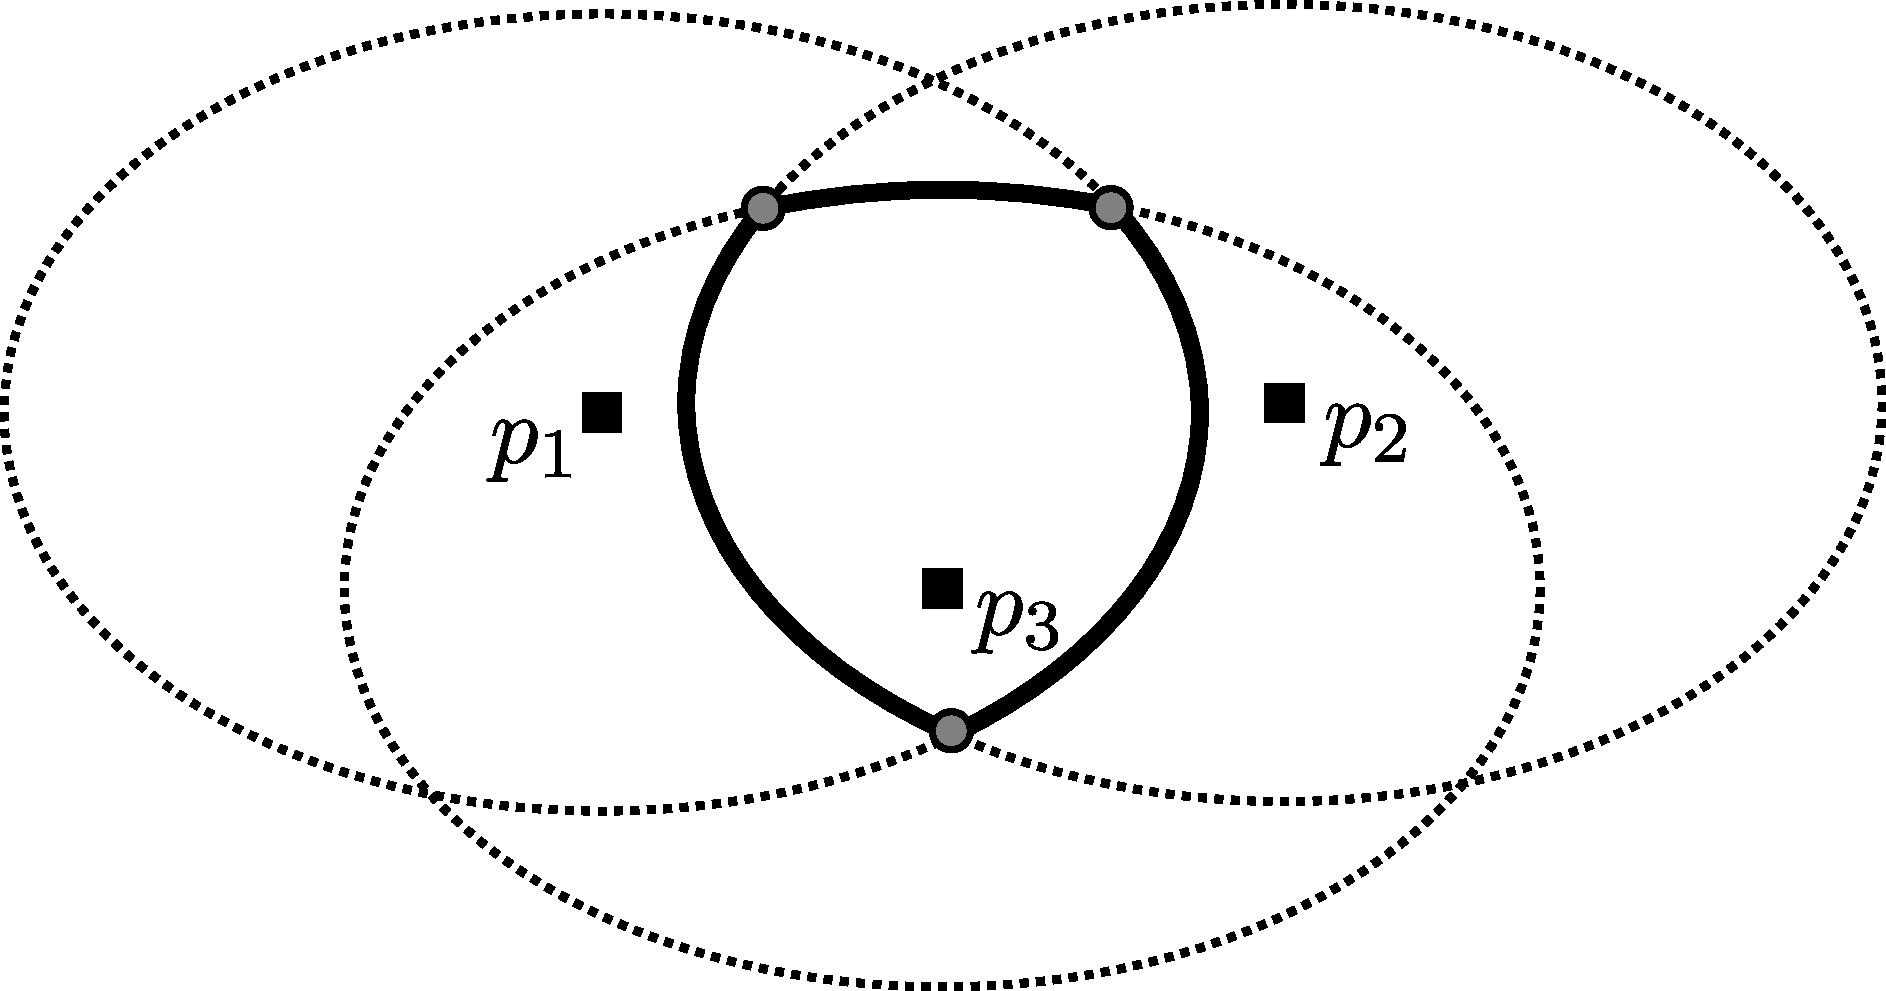
\includegraphics[scale=.3]{figures/MCE-vertices2}
	\caption{Transforming a solution of E3P into a solution of the circumcircle problem.}
	\label{fig:MCE-vertices}
\end{figure}


\begin{lem}\label{lema:e2p}
	Let $E$ be the coverage region of an axis-parallel ellipse with shape parameters $(a,b)$; and $v \in \R^2$, $v\neq0$. Then $|\partial E(0) \cap \partial E(v)| \le 2$, and $\partial E(0) \cap \partial E(v)$ can be determined analytically.
\end{lem}

\begin{proof}
	By \cite{bi}, we have that the number of intersections between two strictly convex circles of fixed radii is at most two. To determine the intersection points, consider the equality between the equations of $\partial E(0)$ and $\partial E(v)$:
	$x^2/a^2 + y^2/b^2 = (x-v_x)^2/a^2 + (y-v_y)^2/b^2.$
	This expression can be reduced to $y=\alpha x + \beta$, for some $\alpha, \beta$. Using $\partial E(0)$'s equation, we obtain at most two values for $x$, which consequently, by $y=\alpha x + \beta$, determine the intersection points between the two ellipses.
\end{proof}

\begin{definition}\label{def:cls_mce}
	Given an instance of MCE, for all $k \in \{1, \dots, m\}$, we define the CLS for the $k$-th ellipse as
	\begin{equation}
	S_k = \Pp \cup \left(\bigcup_{1 \le i < j \le n} \partial E_k(p_i) \cap \partial E_k(p_j) \right).
	\end{equation}
\end{definition}

By \autoref{lema:e2p}, the CLS for each ellipse can be computed in $\bigO(n^2)$, and $|S_k| \le n + 2\binom{n}{2}$. Next, we establish a lemma stating that the set of solutions obtained by combining the possible locations in each ellipse's CLS contains at least one optimal solution.

\begin{thm}\label{thm:mce}
	Given an instance of MCE, and $S_1, \dots, S_m$ as defined by \autoref{def:cls_mce}, then the set $\Omega = \{(q_1, \dots, q_m) \colon \textnormal{ for all }q_k \in S_k \}$ contains an optimal solution of MCE and $|\Omega| \le n^{2m}$. 
\end{thm}
\begin{proof}
	Let $Q^*$ be an optimal solution of MCE for the given instance. Then, we are going to prove that there exists $Q' \in \Omega$, which is also optimal.
	
	For each $k=1, \dots, m$, let $X_k = \{p_i \in \Pp\colon p_i \in E_k(q_k^*)\}$.
	
	%If $|X_k| = 0$, then any $q_k \in S_k$ makes $X_k \subset \Pp \cap E_k(q_k)$.
	
	If $|X_k| \le 1$, then there is at least one element in $S_k$ that makes $X_k \subset \Pp \cap E_k(q_k)$.
	
	If $|X_k| > 1$, then let $Y_k = \cap_{p \in X_k}E_k(p)$. By the results of \cite{bi}, we have that the boundary of $Y_k$ has vertices in the pairwise intersections of $\{\partial E_k(p) \colon p \in X_k\}$. Therefore, at least one vertex of $Y_k$ is in $S_k$, and any of those vertices produce a solution that covers at least the same points covered by $Q^*$.
	
	Lastly, we have that $|S_k| \le 2\binom{n}{2} + n = n(n+1)/2 \le n^2$. Hence, $|\Omega| \le n^{2m}$.
\end{proof}

With all this in hand, we define \autoref{algoritmo:mce}, which goes through every possible combination in the CLS of each ellipse. As evaluating each solution can be done in $\bigO(nm)$, we have that \autoref{algoritmo:mce} has $\bigO(mn^{2m+1})$ runtime complexity. 
In \autoref{section:numerical}, we give more details about the implementation of \autoref{algoritmo:mce} and analyze some numerical experiments for instances proposed in \cite{canbolat, andreta}, and for some new ones.

\begin{algorithm}
	\caption{Algorithm for MCE}\label{algoritmo:mce}
	
	\begin{algorithmic}[1]
		\Require{A set of points $\Pp=\{p_1,\dots,p_n\}$, a list of weights $\Ww=\{w_1, \dots, w_n\}$, and a list of shape parameters $\Rr=\{(a_1, b_1), \dots, (a_m, b_m)\}$.}
		
		\Ensure{An optimal solution for MCE.}
		
		\item[]
		\Procedure{$MCE$}{$\Pp, \Ww, \Rr$}
		\State \Return $MCE_{bt}(\Pp, \Ww, \Rr, 1)$
		\EndProcedure
		\State
		\Procedure{$MCE_{bt}$}{$Z, \Ww, \Rr, j$}
		\If{$j = |\Rr|+1$}
		\State \Return $0$
		\EndIf
		
		\State $(q_j^*, \dots, q_m^*) \gets (0, \dots, 0)$
		\State Let $S_j$ be the CLS for the $j$-th ellipse as defined by \autoref{def:cls_mce}.
		%\State $S_j \gets \textnormal{CLS-MCE}(Z, a_j, b_j)$
		\For{$q_j \in S_j$}
		\State $Cov \gets \Pp \cap E_j(q_j)$
		\State $(q_{j+1}, \dots, q_m) \gets MCE_{bt}(Z \setminus Cov, \Ww, \Rr, j+1)\}$
		
		\If{$w(\cup_{k=j}^m Z \cap E_k(q_k)) >  w(\cup_{k=j}^m Z \cap E_k(q_k^*))$}
		\State $(q_j^*, \dots, q_m^*) \gets(q_j, \dots, q_m)$
		\EndIf
		\EndFor
		
		\State \Return $(q_j^*, \dots, q_m^*)$
		\EndProcedure
	\end{algorithmic}
\end{algorithm}